\documentclass[12pt]{article}
\usepackage{amsmath}
\usepackage{amssymb}
\usepackage{stackrel}
\usepackage{cite}
\usepackage{color}
\usepackage[margin=1in,footskip=0.15in]{geometry}
%\usepackage[]{algorithm2e}
\usepackage{algorithm}
% Need it for floating environment
\usepackage[noend]{algpseudocode}
% Hide endif .etc
\usepackage{caption}
% Need it for \caption*
\usepackage{xspace}
% Fix macro spacing bug
\usepackage[utf8]{inputenc}
\usepackage[english]{babel}
\usepackage{amsfonts}

\usepackage{tikz}
\usepackage{graphicx}
\usetikzlibrary{arrows}
\tikzset{every picture/.style={font issue=\scriptsize},
         font issue/.style={execute at begin picture={#1\selectfont}}}

%-------------------------------------------------------------
\usepackage{float}

\usepackage{algorithm}
\usepackage{algpseudocode} 

\algnewcommand\algorithmicinput{\textbf{Input:}}
\algnewcommand\Input{\item[\algorithmicinput]}

\algnewcommand\algorithmicoutput{\textbf{Output:}}
\algnewcommand\Output{\item[\algorithmicoutput]}

\algnewcommand\algorithmicparameters{\textbf{Parameters:}}
\algnewcommand\Parameters{\item[\algorithmicparameters]}
\renewcommand{\thealgorithm}{\arabic{algorithm}}

\algtext*{EndIf} % Remove "end if" text
\algtext*{EndFor} % Remove "end for" text
\algtext*{EndWhile} % Remove "end while" text
\algtext*{EndFunction} % Remove "end function" text

\renewcommand{\algorithmicrequire}{\textbf{Input:}}
\renewcommand{\algorithmicensure}{\textbf{Output:}}
\renewcommand{\algorithmicensure}{\textbf{Parameters:}}
%%----------------------------------------------------------
%%Macros:
\renewcommand{\j}{j} % index of single-cell
\newcommand{\CN}{C} %copy number (for haplotypes)
\newcommand{\X}{X} % read count
\renewcommand{\d}{d} % direction
\newcommand{\D}{\mathcal{D}} % direction set
\renewcommand{\k}{k} % index of the segment
\newcommand{\h}{h} % haplotype index
\renewcommand{\H}{\mathcal{H}} % haplotype set
\newcommand{\T}{T} % strand state random var
\newcommand{\V}{V} % variation (SV type)
\newcommand{\N}{N} % W and C CN in segment strand patterns
%%----------------------------------------------------------

\newtheorem{theorem}{Theorem}[section]
\newtheorem{definition}[theorem]{Definition}
\newtheorem{proposition}[theorem]{Proposition}

\title{Notations and the statistical model for read count of StrandSeq data}

\begin{document}

\maketitle

\section{Computing Strand-seq read count likelihoods for different Haplotype-aware SV classes}

The read counts in genomic regions are shown to come from a Negative Binomial (NB) distribution \textcolor{red}{cite}. %TODO:FIXME~\citep{nb}.
Given a set of breakpoints and the estimated NB $p$ and $r$ parameters, we compute the likelihood of the observed Watson and Crick read counts per single-cell and segment for each haplotype-resolved SV status.

\subsection{Notations}
We present a set of notations in table~\ref{notations}. $\X$, $\T$ and $\V$ denote read counts and single-cell strand states and SV type, respectively.
Note that a haplotype-resolved SV class can be encoded as the number of normal and inverted copies of a region in each haplotype, which are denoted by $C$ notation.
$S$ denotes the size of a segment, which is defined as the number of bins inside the segment, and $N$ is the number of W and C copy numbers in a segment in a single-cell.

Note that segment strand pattern is differnt from single-cell strand states.
The latter is refered to the inherited strand-state in a single-cell in a chromosome, which can be variable in the range of a chromosome in case an SCE event happens, and it can only have one of the four possible states in $\T = \{CC,CW,WC,WW\}$ for diploid cells.
However, segment strand pattern is a function of single-cell strand state and the SV class in a segment.
For example, if the strand state in a single-cell is $WW$ in a chromosome and an inverted duplication happens in a segment in that chromosome, the strand pattern in that segment will be $WWC$.
Table \textcolor{red}{xxx} shows the values of segment strand patterns for different SV classes and single-cell strand states.

\subsection{Probabilistic model}
The Strand-seq directional read counts in segments are assumed to be generated by the following probabilistic model:
for each single-cell and each segment, the segment Watson and Crick copy number ($N$) is a function of the haplotype-specific single-cell strand state ($T$) and the SV class ($V$) in that segment. The strand pattern of segment $\k$ in single-cell $\j$ ($SP_{\j,\k}$) and the Watson and Crick copy numbers of the segment can be computed as follows:

\begin{align}
	SP_{\j,\k} = {\T^{\stackrel{\rightarrow}\CN_{\j,\k,\h_1}}_{\j, \k, \h_1}}.
				  {\overline{\T}^{\stackrel{\leftarrow}\CN_{\j,\k,\h_1}}_{\j, \k,\h_1}}.
				  \T^{\stackrel{\rightarrow}\CN_{\j,\k,\h_2}}_{\j, \k, \h_2}.
				  {\overline{\T}^{\stackrel{\leftarrow}\CN_{\j,\k,\h_2}}_{\j, \k,\h_2}}\nonumber\\
	\N_{\j, \k}^W = \text{nmuber of W letters in } SP_{\j,\k}\nonumber\\
	\N_{\j, \k}^C = \text{nmuber of C letters in } SP_{\j,\k}\nonumber
\end{align}
where $\overline{\T}$ means the opposite direction for $\T \in \{W, C\}$, dot is the operation for concationating strings, and $\T^C$ means concatenation of $\T$ for $C$ times.

Given the Watson and Crick copy numbers in a segment, we can compute the likelihood of the observed read counts by NB distribution:
\begin{align}
	\X_{\j,\k}^W \sim NB(r_{\j,\k}^W, p)\nonumber\\
	\X_{\j,\k}^C \sim NB(r_{\j,\k}^C, p)\nonumber
\end{align}
where $p$ is the estimated $p$ parameter in NB distribution from bin read counts, and $r_{\j,\k}^W$ and $r_{\j,\k}^C$ are proportional to the estimated parameter $r_\j$, the segment size $L_\k$ and the Watson and Crick segment copy numbers ($\N_{\j, \k}^W$ and $\N_{\j, \k}^W$) and hence are computed as follows:
\[
r_{\j,\k}^d = 
\begin{cases}
\alpha r_\j L_\k &\text{if } \N_{\j, \k}^d = 0 \\ 
(1- \alpha) r_\j L_\k \N_{\j, \k}^d &\text{otherwise}
\end{cases}
\]
In this formula, $\alpha$ is a parameter in our model indicating the fraction of background reads that come from the opposite of the expected direction. These noisy background reads have been observed in Strand-seq data, which is the reason we incorporate this parameter in our model.

To sum up, every haplotype-resolved SV class ($\V$) in a segment together with the haplotype-resolved strand state of a single-cell ($\T$), define a Watson and Crick copy number ($\N$), which will be then used to compute the NB likelihood of the observed read counts.


\begin{figure}
	\begin{center}
		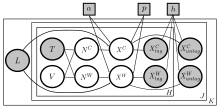
\includegraphics[width=\textwidth]{graphical_model_haplotagged-equal-sized-circle}
	\end{center}
\caption{A graphical model for directional strand-seq read counts in genomic segments resulting from SV classes. $J$, $K$, and $H$ denote the set of single-cells, segments, and haplotypes. $\T_{\h,\k,\j}$ and $\V_{\h,\k,\j}$ respectively denote the strand state and the SV status of haplotype h in segment s in single-cell $\j$. $\N$ denotes a segment strand pattern, i.e., W and C copy numbers in a segment in a single-cell, and $\X^W$ and $\X^C$ denote the W and C read counts (observed) in a segment and a single-cell.}
\end{figure}

\begin{table*}[tb]
	\caption{Overview of notations}
	\centering
	\begin{tabular}{  p{4cm} p{12.5cm} }
		\hline
		Notation & Definition\\
		\hline
		$\X_{\j,\k}^W$ & The number of Strand-seq reads from single cell $\j$ mapped to the $\k$th segment in Watson direction\\

		$\X_{\j,\k}^C$ & The number of Strand-seq reads from single cell $\j$ mapped to the $\k$th segment in Crick direction\\
		
		$\X_{\j,\k}$ & $(\X_{\j,\k}^W, \X_{\j,\k}^C)$\\
		
		$\T_{\j, \k, \h} \in \T$ & The strand state of single cell $\j$ in haplotype $\h$ in the part of chromosome covering segment $\k$\\
		
		$\T_{\j,\k}$ & $(\T_{\j, \k}^{\h_1}, \T_{\j, \k}^{\h_2})$\\
		
		$\stackrel{\rightarrow}{\CN}_{\j,\k,\h}$ & The number of copies of segment $\k$ in single-cell $\j$ and haplotype $\h$ \\
		
		$\stackrel{\leftarrow}{\CN}_{\j,\k,\h}$ & The number of inverted copies of segment $\k$ in single-cell $\j$ and haplotype $\h$ \\
		
		$\V_{\j, \k, \h}$ &$(\stackrel{\rightarrow}{\CN}_{\j,\k,\h}, \stackrel{\leftarrow}{\CN}_{\j,\k,\h})$ : SV type in segment $\k$ in single-cell $\j$ and haplotype $\h$\\
		
		$p$ & The $p$ parameter in NB distribution for the read counts from a single-cell inside a bin for normal copy number 2\\
		
		$r_\j$ & The dispersion ($r$) parameter in NB distribution for the read counts from single-cell $\j$ inside a bin for normal copy number 2\\
		
		$r_{\j,\k}^W$ & The dispersion ($r$) parameter in NB distribution for Watson read counts from single-cell $\j$ in segment $\k$\\
		
		$r_{\j,\k}^C$ & The dispersion ($r$) parameter in NB distribution for Crick read counts from single-cell $\j$ in segment $\k$\\
		
		$L_\k$ & size (number of bins) of segment $\k$\\
		
		$\N_{\j, \k}^W$ & Watson copy number in single-cell $\j$ and segment $\k$\\
		
		$\N_{\j, \k}^C$ & Crick copy number in single-cell $\j$ and segment $\k$\\
		
		$\N_{\j, \k}$ & $(\N_{\j, \k}^W, \N_{\j, \k}^C)$\\
		
		$SP_{\j,\k}$ & $\in \{C,W,CC,WC,WW,CCC,CCW, \cdots\}$ : strand pattern of segment $\k$ in single-cell $\j$\\
		\hline
	\end{tabular}
	\label{notations}\vspace{-4.5mm}
\end{table*}

\section{Haplotagged read count likelihood}
\textcolor{red}{
Haplotype-phasing. MosaiCatcher phases Strand-seq data using StrandPhaseR39, based on the principle that in ‘WC’ chromosomes reads (and SVs) can be readily separated into chromosome-length haplotypes.}

\bibliographystyle{natbib}
% \bibliographystyle{achemnat}
% \bibliographystyle{plainnat}
% \bibliographystyle{abbrv}
% \bibliographystyle{bioinformatics}

\bibliographystyle{plain}

\bibliography{document}

\end{document}